\documentclass{article}

% Packages
\usepackage{graphicx} % For including images
\usepackage{amsmath} % For mathematical symbols and equations

% Title and Author Information
\title{Model Stealing Attack}
\author{Byung Jae Bae}
\date{\today}

\begin{document}

\maketitle

\begin{abstract}
    This is the abstract of your article. Provide a brief summary of your work and its key findings.
\end{abstract}

\section{Introduction}
We run a KnockoffNet attack on a pretrained Resnet50 model trained on the CIFAR dataset with another Resnet50 model but trained on both 
CIFAR and MNIST datasets. We test the new KnockoffNet trained on 10k, 20k, 30k, 40k, and 50k queries to the original pretrained model on the 
CIFAR test dataset, MNIST test dataset, and both combined CIFAR and MNIST test dataset to compare the how the different datasets affect the test accuracies.

\section{Results}
The accuracies of the CIFAR test dataset for 10k, 20k, 30k, 40k, and 50k queries were 0.137, 0.1154, 0.151, 0.1797, and 0.161, respectively.
For the MNIST and CIFAR dataset it was 0.1984, 0.18735, 0.18895, 0.23545, and 0.21055.
For only MNIST it was 0.189, 0.1795, 0.1488, 0.2127, 0.2185. The table below makes a clearer illustration.

\begin{figure}
    \begin{center}
        \begin{tabular}{|c | c c c|} 
        \hline
        Number of Queries & CIFAR & MNIST and CIFAR & MNIST \\ [0.5ex] 
        \hline
        10000 & 0.137 & 0.1984 & 0.189 \\ 
        \hline
        20000 & 0.1154 & 0.18735 & 0.1795 \\
        \hline
        30000 & 0.151 & 0.18895 & 0.1488 \\
        \hline
        40000 & 0.1797 & 0.23545 & 0.2127 \\
        \hline
        50000 & 0.161 & 0.21055 & 0.2185 \\ [1ex] 
        \hline
        \end{tabular}
    \end{center}
    \caption{Table of accuracies for different number of queries.}
    \label{fig:table1}
\end{figure}


\begin{figure}
    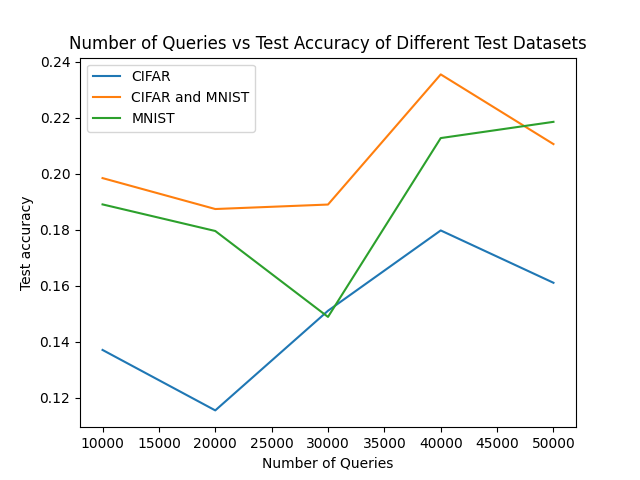
\includegraphics[width=\linewidth]{acc.png}
    \caption{Graph of accuracies for different number of queries.}
    \label{fig:graph1}
\end{figure}

\section{Discussion}
The results were somewhat surprising. Firstly, the accuracies for all test accuracies were very low even for 50k queries.
Secondly, there were no linear trends between number of queries and test accuracies, as the test accuracies would fluctuate throughout
the different query numbers.
\section{Conclusion}
Summarize the key points of your article and discuss possible future research directions.

\section*{Acknowledgments}
You can acknowledge individuals or organizations that contributed to your work.

\section*{References}
Include references to the sources cited in your article. You can use tools like BibTeX or manually create the bibliography.

% Example of citing a reference
% \cite{example_reference}

\end{document}